%\section{Аналіз існуючих моделей і алгоритмів управління логістичними системами. Постановка задачі}
\section{Аналіз предметної області}
\subsection{Розподільча логістична система як об'єкт дослідження}
\subsubsection{Сутність розподільчої логістики}
% http://studentbooks.com.ua/content/view/126/76/1/25/#242234
Оскільки розподільча логістика тісно пов’язана зі збутом продукції, необхідно зупинитися на його завданнях.

Щоб зрозуміти сутність збутової орієнтації товаровиробників, розглянемо складові збутової діяльності. 
Під збутовою діяльністю слід розуміти процес організації товарного обміну готової продукції з метою одержання підприємницького прибутку. 
Під готовою продукцією розуміють вироби, роботи, послуги, що завершені виробництвом на даному підприємстві і можуть бути запропоновані ринку. 
Цілі збуту виходять з цілей підприємства, серед яких зараз превалюють цілі максимізації прибутку. 
Враховуючи практику одержання спекулятивного прибутку, слід ідентифікувати природу прибутку від збутової діяльності як підприємницький прибуток. 
При цьому переслідується така мета:
\begin{itemize}
	\item освоєння ринку;
	\item збереження ринку;
	\item вичерпання ринку.
\end{itemize}

Слід враховувати й існування виробничих процесів.

Основними елементами збуту вважаються системи збуту, форми збуту та шляхи збуту. 
Сполучення цих складових у різних ринкових ситуаціях дають можливість фірмі-товаровиробнику ефективно реалізувати відповідні цілі збуту. 
Самі ж елементи збуту, сполучення котрих обирають, формуючи відповідний метод збуту, являють собою структуру розподілу основних функцій збуту~(рисунок~\ref{fig:sales_functions}).

\begin{figure}
	\centering
	\begin{tikzpicture}
		\node at (-3,0) {Планування};
		\node at (-6,-5.5) {Організація};
		\node at (-1,-5.5) {Контроль та регулювання};
		\node at (-3,-3.5) {Збут};
		\draw (-3,-0.5) node (v1) {} -- (-5.5,-5) -- (-0.5,-5) -- cycle;
	\end{tikzpicture}
	\caption{Основні функції збуту}
	\label{fig:sales_functions}
\end{figure}

Функції планування:
розробка перспективних та оперативних планів продажу, 
аналіз і оцінка кон'юнктури ринку, 
визначення споживацького попиту, 
формування асортиментного плану виробництва за замовленнями покупців, 
вибір каналів та товароруху, 
планування рекламних кампаній і розробку заходів стимулювання збуту, 
укладання кошторисів-витрат для цілей збуту та їх оптимізація.

Функції організації:
організація складського і тарного господарства для готової продукції, 
організація продажу і доставки продукції споживачам, 
організація допродажного і післяпродажного обслуговування споживачів, 
організація каналів товароруху і розподільчих мереж, 
організація проведення рекламних кампаній та заходів стимулювання збуту, 
організація підготовки торговельного персоналу та управління діяльністю торговельних представництв, 
організація взаємодії всіх підрозділів підприємства для досягнення цілей збуту.

Функції контролю та регулювання:
оцінка результатів діяльності,
контроль за виконанням планів,
оперативне регулювання збутовою діяльністю підприємства з урахуванням впливу зовнішніх та внутрішніх чинників,
оцінка і стимулювання діяльності збутового апарату,
статистичний, бухгалтерський та оперативний облік збутової діяльності.

Збутова орієнтація підприємства передбачає певним чином організовану роботу всіх його підрозділів та служб, що може бути успішно досягнуто на основі логістичного моделювання.

Успіх використання логістичного підходу у виробництві зумовлений перевагами логістичного підходу до організації збуту у порівнянні з традиційним. 
Переваги логістичного підходу полягають у тому, що логістика повною мірою <<працює>> перш за все на споживача. 
Успіхи логістики пов’язані з її використанням у високорозвинутій ринковій економіці, де товарність досягла свого найвищого рівня. 
Об’єктивна необхідність логістики як нової науки виникла у зв’язку із закономірним розвитком ринкової економіки розвинутих країн перш за все з її переходом від локальних господарчих систем до інтегрованих структур, що поєднують у межах єдиних логістичних систем функції постачання виробництва, транспорту, розподілу і ринку на основі потужної виробничої інфраструктури. 
На відміну від старих методів і форм управління спеціалізованими господарчими системами чи окремими функціями і ділянками внутрішньогосподарських систем логістика дозволяє координоване управління матеріальними та інформаційними потоками, забезпечуючи їх синхронність та високі кінцеві результати діяльності всіх ділянок товароруху.

Різноманітність стратегічних і оперативних завдань підприємства висуває перед розподільчою логістикою проблему визначення пріоритетів їх вирішення, що можливо успішно виконати за наявності критерію оптимальності чи цільової функції. 
Найчастіше цільовою функцією розподільчої логістики виступає максимізація прибутку підприємства при повному задоволенні платоспроможного попиту споживачів. 
У процесі перевірки завдань за цільовою функцією здійснюється їх ранжування та вибракування неефективних напрямів збутової діяльності і несуттєвих для підприємства проблем.

Поняття розподілу у комерційній діяльності, в тому числі й збутову, має два смислових значення:
\begin{itemize}
	\item узгодження, розміщення і доставки товарів; 
	\item весь комплекс операцій, що здійснюються з метою доставки товарів та послуг споживачам. 
\end{itemize}

% https://essuir.sumdu.edu.ua/bitstream/123456789/38038/1/Bilovodska_Kyslyi_Olefirenko_Solyanyk.pdf
Розподільча логістика --- це частина загальної логістичної системи, яка забезпечує найбільш ефективну організацію розподілу продукції, охоплюючи систему товароруху і виконуючи логістичні операції транспортування, складування, упакування та ін.~\cite{Kusluy2010}.

Розподільча логістика спрямована на комплексне планування, управління та фізичне опрацювання потоку готових виробів у супроводі необхідного інформаційного, фінансового та сервісного потоку від моменту здачі-приймання товарів з виробництва до замовника (споживача) з метою оптимізації витратних та часових характеристик зазначеної частини матеріального і нематеріального потоків.
Головна мета розподільчої логістики --- організація розподільчої діяльності відповідно до замовлень клієнтів з мінімальними загальними витратами~\cite{Kusluy2010}.

Принципова відмінність розподільчої логістики від традиційного розуміння збуту полягає насамперед у системному взаємозв'язку процесу розподілу з процесами виробництва і закупівель під час управління матеріальними потоками, а також системному взаємозв'язку всіх функцій всередині самого розподілу.

Матеріальний потік у сфері розподілу має форму готової продукції.
Залежно від суб'єкту економічних відносин, який бере участь у доведенні ресурсів до споживача, потік готової продукції можна подати як товарний потік або як вантажний потік (на транспорті).

Розподільча логістика будується на загальних логістичних принципах~\cite{Anikin1999}:
\begin{itemize}
	\item координація всіх процесів товароруху, починаючи від кінцевих операцій товаровиробника та закінчуючи сервісом споживача;
	\item інтеграція всіх функцій управління процесами розподілу готової продукції та послуг, починаючи від визначення мети та закінчуючи контролем;
	\item адаптація комерційного, канального та фізичного розподілу до постійно змінних вимог ринку та потреб споживача;
	\item координація всіх процесів товароруху, починаючи від кінцевих операцій товаровиробника та закінчуючи сервісом споживача;
	\item системність як управління розподілом в його цілісності та взаємозалежності всіх елементів збутової діяльності;
	\item комплексність, тобто вирішення всієї сукупності проблем, пов’язаних із задоволенням платоспроможного попиту покупців;
	\item оптимальність стосовно як елементів системи, так і режиму її функціонування;
	\item раціональність як в організаційній структурі, так і в організації управління.
\end{itemize}

Склад завдань розподільчої логістики на мікро- та на макрорівні різний~(таблиця~\ref{tab:logistic_functions}). 

\begin{table}[H]
	\caption{Завдання розподільчої логістики на мікро- та макрорівнях}
	\label{tab:logistic_functions}
	\begin{tabular}{@{}|p{0.53\linewidth}|p{0.4\linewidth}|@{}}
	 	\hline
		Мікрорівень & Макрорівень \\ \hline
		\begin{itemize}[leftmargin=*]
			\item оптимізація формування портфеля замовлень;
			\item укладання договорів із замовниками на постачання продукції;
			\item забезпечення ритмічності та дотримання планомірності реалізації продукції;
			\item вивчення і задоволення потреб у логістичному сервісі;
			\item раціоналізація параметрів, структури і просування динамічних матеріальних потоків;
			\item оптимізація параметрів і умов зберігання запасів товарного характеру;
			\item формування і вдосконалення системи інформаційного забезпечення.
		\end{itemize}
		&
		\begin{itemize}[leftmargin=*]
			\item вибір схеми розподілу матеріального потоку;
			\item визначення оптимальної кількості розподільчих центрів на території, яка обслуговується;
			\item визначення оптимального місця розташування розподільчого центру на території, яка обслуговується, та ін.
		\end{itemize} \\ \hline
	\end{tabular}
\end{table}

\subsubsection{Канали розподілу в логістиці}
Канал розподілу --- це сукупність підприємств і організацій, через які проходить продукція від місця її виготовлення до місця споживання. 
Іншими словами канал розподілу --- це шлях, яким товари переміщуються від виробника до споживача.

Залежно від розмірів, потужності підприємства-виробника, різноманітності продукції та інших факторів, товаропровідна мережа може складатися із одного, декількох або багатьох каналів розподілу, причому різні канали розподілу товарів можуть відрізнятися за структурою, типами торгових посередників і проміжних складів, способами доставки вантажів, видами транспорту і т.д. 
Сукупність каналів розподілу називається розподільчою мережею.

З позицій виробників, які генерують матеріальні потоки; чим більше рівнів має логістичний канал, тим більше труднощів в узгодженості функціонування всіх ланок з просування матеріальних потоків до споживачів.
Канали розподілу можуть бути горизонтальними і вертикальними.

Горизонтальні канали розподілу є традиційними каналами і складаються із незалежного виробника та одного або декількох незалежних посередників. 
Кожен член каналу є окремим підприємством, яке прагне забезпечити собі максимальний прибуток. 
Максимально можливий прибуток окремого члена каналу може завдавати шкоди отриманню максимального прибутку системою в цілому, оскільки жоден із членів каналу не має повного або достатнього контролю над діяльністю решти членів.

Вертикальні канали розподілу --- це канали, які складаються з виробника та одного або декількох посередників, які діють як одна єдина система. 
Один із членів каналу, як правило, або є власником інших, або надає їм певні привілеї. 
Таким членом може бути виробник, оптовий або роздрібний посередник. 
Вертикальні канали виникли як засіб контролю за поведінкою каналу. 
Вони економічні та виключають дублювання членами каналу виконуваних функцій.

Проблема управління каналами розподілу полягає в тому, що посередницькі структури, що займають проміжне становище між виробниками і споживачами, не завжди прагнуть до зміцнення взаємозв'язків із продуцентами. 
Вони віддають перевагу більш тісним контактам із споживачами. 
Більшість посередницьких структур хочуть, аби виробники доводили матеріальні потоки до них і не втручалися в логістичні процеси на подальших етапах переміщення цих потоків. 
Підставою для цього служить те, що нерідко на практиці виробники товарної продукції ставляться до логістичних посередників гірше, ніж до кінцевих споживачів, запити, мотивація і очікування яких вивчаються і задовольняються. 

\subsection{Проблеми моделювання і управління розподільчими логістичними системами}
Основною проблемою, характерною для об'єкта дослідження, яка породжує безліч інших проблем, є його ієрархічність і розподіленість. 
В таких системах процеси розосереджені по окремих підсистемах і знаходяться на різних рівнях ієрархії. 
Для таких систем вирішується комплекс взаємопов'язаних задач в режимі багатосторонньої взаємодії між менеджерами-аналітиками, що відповідають за окремі локальні завдання і ЕОМ. 
Їх знання, компетенція, функції та відповідальність розосереджені по окремих етапах і робочих місць, які пов'язані як <<по вертикалі>>, так і <<по горизонталі>>.
Основними ознаками розподіленості будь-якої логістичної системи можна вважати:
\begin{itemize}
	\item наявність механізму розбиття даної системи на окремі взаємопов'язані підсистеми;
	\item окремі складові системи географічно відокремлені;
	\item відносна автономність окремих підсистем;
	\item спільне завдання всієї системи розглядається у вигляді набору окремих локальних підзадач;
	\item паралельність і асинхронність рішення окремих локальних задач різними виконавцями.
\end{itemize}

Першою проблемою, яку необхідно вирішувати, є розбиття кожної системи на окремі локальні підсистеми. 
Можна сказати, що формалізація цих двох завдань здійснюється на основі декомпозиції і агрегування. 
Декомпозиція полягає в розчленуванні вихідної задачі на ряд відносно незалежних підзадач, а агрегування --- в заміні окремих груп змінних, що характеризують ефективність функціонування системи, змінними-агрегатами. 
При цьому висувається вимога повної (достатньої) еквівалентності задач. 
Агрегування параметрів і змінних здійснюється в ході руху вгору по ієрархії. 
Це пов'язано з великою розмірністю завдання і неможливістю прийняття рішень на основі варіювання всіх параметрів і змінних. 
Основні ідеї, які реалізуються при синтезі моделі на основі декомпозиції і агрегування полягають у наступному:
\begin{itemize}
\item нехтуючи слабкими зв'язками між окремими підсистемами, зробити декомпозицію;
\item використовуючи трохи відмінності між ними, зробити агрегування;
\item використовуючи сильні відмінності, виділити <<вузькі місця>>, відкинувши на основі апріорних оцінок несуттєві обмеження.
\end{itemize}

\subsection{Моделі логістичних систем}
Необхідність широкого використання моделювання у розподільчій логістиці пояснюється як складністю збутової діяльності, так і основним засобом розподілу --- логістичним моделюванням. 
У розподільчій логістиці успішно можуть бути використані такі моделі, як:
\begin{itemize}
	\item моделі теорії ігор; 
	\item моделі теорії черг або теорії масового обслуговування;
	\item моделі управління запасами;
	\item моделі лінійного програмування;
	\item імітаційне моделювання тощо.
\end{itemize}

Одним з найбільш ефективних методів дослідження складних систем є імітаційне моделювання~\cite{Kobelev2003}.

<<Імітація>> означає відтворення певним чином явищ, подій, дій, об'єктів і т. п.~\cite{Kobelev2003}. 
Цей термін є синонімом поняття <<модель>> — абстрактний опис системи (об'єкта, процесу, проблеми, поняття) в деякій формі, відмінній від форми її реального існування~\cite{Emelyanov2002}. 

Моделювання в загальному вигляді являє собою один з основних методів пізнання, є формою відображення дійсності і полягає у з'ясуванні або відтворенні тих чи інших властивостей реальних об'єктів, процесів, явищ за допомогою абстрактного опису у вигляді зображення, плану, карти, сукупності рівнянь, алгоритмі і програм.

Імітаційне моделювання --- експериментальний метод дослідження реальної системи за її імітаційною моделлю, який поєднує особливості експериментального підходу і специфічні умови використання обчислювальної техніки~\cite{Emelyanov2002}.

Серед переваг імітаційного моделювання відзначають~\cite{Emelyanov2002}: 
\begin{enumerate}
	\item Відображення динамічних процесів і поведінкових аспектів зовнішнього середовища.
	\item Можливість виявлення закономірностей, динамічних тенденцій розвитку і функціонування складної системи в умовах неповної та неточної інформації.
	\item Опис взаємодії та поведінки безлічі активних агентів в соціальних системах.
	\item Реалізацію принципів об'єктно-орієнтованого проектування і застосування високотехнологічних рішень при побудові комп'ютерних моделей та ін.
\end{enumerate}

Головною проблемою при побудові будь імітаційної моделі є необхідність побудови комплексних математичних моделей і розробки програмного коду імітаційної моделі. 

У імітаційному моделюванні виділяють такі основні підходи:
\begin{itemize}
	\item системна динаміка;
	\item дискретне моделювання;
	\item агентне моделювання.
\end{itemize}

Як методологія системна динаміка була запропонована в 1961 році Дж. Форрестером в якості інструменту дослідження інформаційних зворотних зв'язків у виробничо-господарської діяльності. 
Процеси, що відбуваються в реальному світі, в системній динаміці представляються в термінах накопичувачів і потоків між ними.
Системнодинамічна модель описує поведінку системи та її структуру як безліч взаємодіючих зворотних зв'язків і затримок. 
Математично така модель виглядає як система диференціальних рівнянь. 
Результатом моделювання в системній динаміці є виявлення глобальних залежностей і причинно-наслідкових зв'язків у досліджуваній системі~\cite{Shamrin2016}. 

Основний об'єкт в системі дискретного моделювання --- пасивний транзакт, який може певним чином представляти собою працівників, деталі, сировину, документи, сигнали і т. п.
Переміщаючись по моделі, транзакти стають в черги до одноканальним і багатоканальним пристроям, захоплюють і звільняють їх, розщеплюються, знищуються і т. д.
Відмінною особливістю даного підходу є час просування по моделі: або від події до події, або через дискретні проміжки часу. 
Дискретне моделювання застосовується, якщо можливо припустити, що змінні в системі змінюються миттєво в певні проміжки часу. 
Даний підхід імітаційного моделювання є одним з найпоширеніших і застосовується для дослідження соціально-економічних, технічних, логістичних та інших процесів.
На основі дискретного підходу реалізовано найбільше
число систем імітаційного моделювання~\cite{Shamrin2016}. 

Агентське моделювання з'явилося в 90-х роках і використовується для дослідження децентралізованих систем, динаміка функціонування яких визначається не глобальними правилами і законами (як в інших парадигмах моделювання), а коли ці глобальні правила і закони є результатом індивідуальної активності членів групи.

Агентно-орієнтована система може складатися з одного агента (наприклад, програмний секретар~\cite{Maes1995}), проте весь потенціал розкривається з використанням мультиагентної системи~\cite{Waters1989}.
Під агентом розуміється система, яка має такі властивості~\cite{Jennings1998,Wooldridge1995}:
\begin{enumerate}[label={\arabic*)}]
	\item автономність: агенти мають внутрішній стан (який недоступний іншим агентам) та приймають рішення на основі своїх даних, без прямого втручання людини;
	\item реактивність: агенти розміщуються в навколишньому середовищі (яке може бути фізичним світом, множиною інших агентів, інтернетом і т.д.), здатні спостерігати і своєчасно реагувати на зміни;
	\item проактивність: агенти не тільки реагують на зміни в зовнішньому середовищі, вони здатні виявляти ініціативу для досягнення своєї мети;
	\item соціальність: агенти взаємодіють з іншими агентами (і, можливо, людиною) через спеціальний інтерфейс для досягнення їх цілей.
\end{enumerate}

Мета агентських моделей --- отримати уявлення про ці глобальні правила, загальну поведінку системи, виходячи з припущень про індивідуальну, приватну поведінку її окремих активних об'єктів і взаємодію цих об'єктів в системі.
У разі моделювання логістичних систем, що містять великі кількості активних об'єктів (людей, машин, підприємств чи навіть проектів, активів, товарів і т. п.), які об'єднує наявність елементів індивідуальної поведінки, агентське моделювання є підходом більш універсальним і потужним, оскільки дозволяє врахувати будь-які складні структури та їх поведінку~\cite{Shamrin2016}. 

\subsection{Огляд існуючих технологій побудови мультиагентної системи}
Існує велика кількість різноманітних агентних платформ, які значно спрощують розробку \acrshort{mas}~\cite{Kravari2015}.
При реалізації \acrshort{mas} можна виділити два основних підходи до розробки~\cite{Zhou2010}:
\begin{enumerate}[label={\arabic*)}]
	\item програмування агентної системи за допомогою \acrshort{fipa} фреймворків;
	\item використання графічних пакетів розробки для побудови \acrshort{mas}.
\end{enumerate}

Нижче наведено огляд основних технологій побудови \acrshort{mas}. 
У таблиці~\ref{tab:mas_platform_comparsion} приведено порівняння цих платформ.

\subsubsection{Agent Factory}
Agent Factory --- це відкритий набір бібліотек, платформ та мов програмування для розробки (ліцензія LGPL) \acrshort{mas}. 
Фреймворк розділений на дві частини: агенти для комп'ютерів (Agent Factory Standard Edition) та агенти для мобільних пристроїв (Agent Factory Micro Edition)~\cite{Kravari2015}.

Архітектура фреймворку представлена на рисунку~\ref{fig:agentfactory_architecture}

\begin{figure}[H]
	\centering
	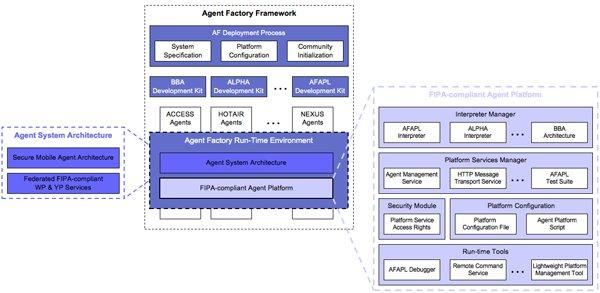
\includegraphics{agentfactory_architecture}
	\caption{Архітектура фреймворку Agent Factory~\cite{agentfactory}}
	\label{fig:agentfactory_architecture}
\end{figure}

Переваги Agent Factory~\cite{Kravari2015}:
\begin{enumerate}[label={\arabic*)}]
	\item швидкість;
	\item відкритість;
	\item проактивність;
	\item сумістність з \acrshort{fipa};
	\item мобільні застосунки.
\end{enumerate}

Недоліками Agent Factory є мала кількість робіт, пов'язаних з розробкою з використанням цього фреймворку, відсутність реалізації бібліотеки візуалізації стану агентної системи, яка є необхідною при побудові аналітичної системи~\cite{Kravari2015}. 
Остання версія цього фреймвроку вийшла в 2016 році.

\subsubsection{JADE}
\acrshort{jade} --- безкоштовна для використання платформа з відкритим вихідним кодом (ліцензія LGPL), написана на Java.
\acrshort{jade} є найпопулярнішою платформою в академічному та промисловому середовищі, що відповідає специфікаціям \acrshort{fipa}.
Система, яка побудована на \acrshort{jade}, може працювати в гетерогенних розподілених системах та віддалено керуватися за допомогою системного інтерфейсу користувача.
\acrshort{jade} потребує \acrshort{jre} версії 1.2 і може бути адаптован для запуску на пристроях з обмеженими ресурсами, таких як мобільні телефони~\cite{Kravari2015}.

\acrshort{jade} платформа складається з контейнерів агентів. 
Контейнери --- це окремі Java процеси які надають середовище \acrshort{jade} та всі сервіси для розміщення та виконання агентів. 
Головний контейнер представляє собою початкову точку платформи --- це перший контейнер, що буде запущений та контейнер, який реєструє всі інші контейнери~\cite{Bellifemine2007}.

Відношення між основними архітектурними елементами системи представлено на рисунку~\ref{fig:jade_architecture}.

\begin{figure}[H]
	\centering
	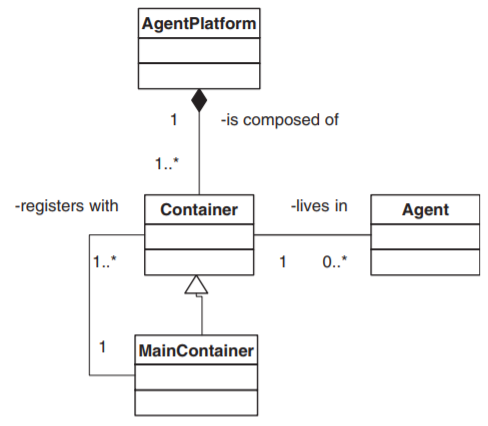
\includegraphics[width=.6\linewidth]{jade_architecture}
	\caption{Відношення між основними архітектурними елементами \acrshort{jade}~\cite{Bellifemine2007}}
	\label{fig:jade_architecture}
\end{figure}

На рисунку~\ref{fig:jade_agent_life_cycle} представлений життєвий цикл агенту за специфікацією \acrshort{fipa}. Агент \acrshort{jade} може знаходитися у одному зі станів, згідно з життєвим циклом агентної платформи~\cite{fipa}:
\begin{itemize}
	\item \texttt{AP\_INITIATED} --- агент створений, але поки що не зареєстрований, тому він не має ані імені, ні адреси та не може обмінюватися повідомленнями з іншими агентами; 
	\item \texttt{AP\_ACTIVE} --- агент зареєстрований, має постійне ім'я та адресу;
	\item \texttt{AP\_SUSPENDED} --- агент у даний момент часу зупинений;
	\item \texttt{AP\_WAITING} --- агент блокований (у очікуванні) до виконання якоїсь дії (наприклад, надходження повідомлення);
	\item \texttt{AP\_DELETED} --- агент більше не зареєстрований у системі;
	\item \texttt{AP\_TRANSIT} --- мобільний агент переміщується до нового місцезнаходження; 
	\item \texttt{AP\_COPY} --- створення копії агента; 
	\item \texttt{AP\_GONE} --- мобільний агент перемістився до нового місцезнаходження, та знаходиться у стійкому стані.
\end{itemize}

\begin{figure}[H]
	\centering
	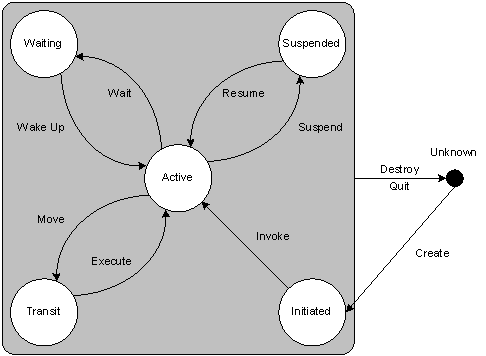
\includegraphics[width=.6\linewidth]{jade_agent_life_cycle}
	\caption{Життєвий цикл агенту за специфікацією \acrshort{fipa}~\cite{fipa}}
	\label{fig:jade_agent_life_cycle}
\end{figure}

Переваги \acrshort{jade}~\cite{Bellifemine2003}:
\begin{enumerate}
	\item Комунікація та координація агентів. \acrshort{jade} спрощує розробку додатків, які вимагають комунікації та координації агентів, де ресурси та структури розподілені у навколишньому середовищі.
	\item Відкритість. \acrshort{jade} --- це проект з відкритим вихідним кодом (LGPL), який включає в себе внески спільноти. 
	\item Проактивність. Агенти \acrshort{jade} можуть легко бути запрограмовані на ініціювання дій. 
	\item Гнучкість. \acrshort{jade} забезпечує однорідний набір \acrshort{api}-інтерфейсів, незалежний від системи.
	\item Розподілена архітектура. Агенти \acrshort{jade} можуть взаємодіяти між собою без центрального серверу. 
	\item Мобільні застосунки. Агенти \acrshort{jade} можуть виконуватись на мобільних пристроях.
	\item Сумісність \textit{(interoperability)}. Платформа \acrshort{jade} відповідає специфікаціям \acrshort{fipa}, а отже є сумісним з агентами інших платформ.
\end{enumerate}

Недоліками \acrshort{jade} є складність процесу розробки та великими трудовитратами на нього. 
Недоліком також є відсутність реалізації бібліотеки візуалізації стану агентної системи, яка є необхідною при побудові аналітичної системи~\cite{Kravari2015}.

\subsubsection{AnyLogic}
AnyLogic --- це програмний засіб для імітаційного моделювання. 
Поєднує в собі графічне середовище для побудови \acrshort{mas} на базі Eclipse та можливість їх програмування на Java~\cite{anylogic,Kravari2015}.

Архітектура AnyLogic представлена на рисунку~\ref{fig:anylogic_architecture}.

\begin{figure}[H]
	\centering
	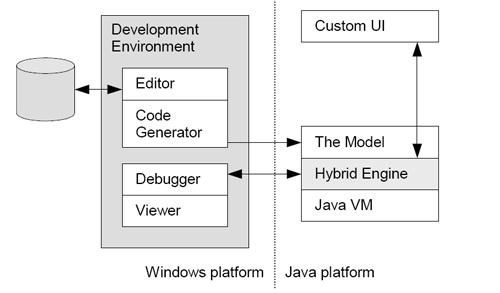
\includegraphics[width=.6\linewidth]{anylogic_architecture}
	\caption{Архітектура середовища моделювання та симуляції AnyLogic~\cite{Borshchev2002}}
	\label{fig:anylogic_architecture}
\end{figure}

Моделі в AnyLogic можуть базуватися на будь-якій з основних парадигм імітаційного моделювання: \acrshort{am}, системній динаміці чи дискретно-подійному моделюванні. 
Також можна поєднувати концепції та засоби з різних підходів моделювання, наприклад, в агентній моделі можна використовувати методи системної динаміки для представлення змін станів середовища, в неперервній моделі динамічної системи врахувати дискретні події.
Наприклад, управління ланцюгами поставок за допомогою імітаційного моделювання вимагає опису учасників ланцюгу поставок агентами: виробники, продавці, споживачі, мережа складів. 
При цьому виробництво описується в рамках дискретно-подійного (процесного) моделювання, продукт чи його частини --- заявки, автомобілі, поїзди --- ресурси. 
Самі поставки представляються дискретними подіями, але при цьому попит на товари може описуватися неперервною системно-динамічною діаграмою. 
Можливість змішувати підходи дозволяє описувати процеси реального життя, а не підганяти процес під доступний математичний апарат~\cite{anylogic,Kravari2015}.

Графічне середовище AnyLogic включає в себе наступні компоненти~\cite{anylogic}:
\begin{enumerate}
\item Stock \& Flow Diagrams (діаграма потоків та накопичувачів) використовується при розробці моделей системної динаміки.
\item Statecharts (діаграми станів) використовуються в агентних моделях для визначення поведінки агентів.
\item Action charts (блок-схеми) використовуються для побудови алгоритмів як в дискретно-подійному моделюванні, так і в агентному моделюванні.
\item Process flowcharts (діаграми процесів) основна конструкція, що застосовується для визначення процесів в дискретно-подійному моделюванні.
\end{enumerate}

Переваги AnyLogic~\cite{anylogic}:
\begin{enumerate}
	\item Середовище багатопідхідного моделювання.
	\item Інтеграція з ГІС-картами.
	\item Запуск моделей в хмарі.
	\item Потужний набір готових експериментів для дослідження моделі під різними кутами.
\end{enumerate}

Недоліками AnyLogic є висока вартість комерційної ліцензії, несумістність з стандартом \acrshort{fipa}.

\subsection{Глосарій проекту}
Глосарій проекту --- це розвернутий словник у вигляді таблиці, який складається з термінів що характеризують дану предметну область.

Глосарій проекту:
\begin{enumerate}
    \item Агент \textit{(agent)} --- це сутність, що спостерігає за навколишнім середовищем і діє у ньому, при цьому його поведінка раціональна в тому розумінні, що він здатен до розуміння і його дії завжди спрямовані на досягнення якої-небудь мети~\cite{Jennings1998}.
    \item Транспорт \textit{(transport)} --- сукупність засобів, для переміщення людей, вантажів, сигналів та інформації з одного місця в інше.
    \item Склад \textit{(warehouse)} --- це складна технічна споруда, яка складається із взаємопов'язаних елементів, що має певну структуру та виконує ряд функцій з перетворення матеріальних потоків, а також накопичення, переробки та розподілу вантажів між споживачами~\cite{Kusluy2010}. 
	\item Запаси гарантійні \textit{(insurance stocks)} призначені для безперервного постачання споживачів у випадку непередбачених обставин: відхилення в періодичності та величині партій поставок від запланованих, зміни інтенсивності споживання, затримки поставок та ін. і є постійною величиною, що залежить від умов виконання конкретних поставок~\cite{Kusluy2010}. 
	\item Ланцюг логістичний \textit{(logistics chain)}  --- це складна система, що формується впорядкованою і взаємодіючою сукупністю фізичних чи юридичних осіб на ринку виробництва і постачання матеріальних ресурсів, виробництва та розподілу продукції, які виконують логістичні операції, спрямовані на доведення матеріального потоку від однієї логістичної системи до іншої та до кінцевого споживача~\cite{Kusluy2010}.  
    \item Логістика \textit{(logistics)} --- системоохоплюючий механізм, який можна трактувати як досягнення компромісу (узгодження) між виконанням зобов’язань і необхідними для цього витратами в сфері виробництва, транспортно-складського забезпечення, у процесі отримання потрібних товарів або послуг у потрібному місці, у потрібний час, у необхідній кількості з мінімальними загальними витратами при високій якості обслуговування споживача~\cite{Kusluy2010}.
	\item Логістика розподільча \textit{(distribution logistics)} --- галузь логістики, яка забезпечує найбільш ефективну організацію розподілу продукції, охоплюючи систему товароруху і виконуючи логістичні операції транспортування, складування, упакування та ін.~\cite{Kusluy2010}.
    \item Операції логістичні \textit{(logistic operations)} --- відособлена сукупність дій, скерована на перетворення матеріального та супутніх йому потоків~\cite{Kusluy2010}.
    \item Сервіс логістичний \textit{(logistic service)} --- це сукупність функцій і видів діяльності всіх підсистем підприємства, що забезпечують зв’язок <<підприємство-споживач>> для кожного матеріального та інформаційного потоку за показниками номенклатури, якості, кількості, ціни, місця і часу постачання продукції відповідно до вимог ринку~\cite{Kusluy2010}.
\end{enumerate}

\subsection{Постановка задачі}
Завданням курсової роботи є розробка мультиагентної системи для дослідження розподільчої логістичної системи.
Задачами є:
\begin{itemize}
	% logistics
	\item опис динаміку розподільчої логістичної системи;
	\item дослідження проблеми імітаціонного моделювання розподільчої логістичної системи;
	% agents
	\item порівняти фреймворки для реалізації мультиагентних систем, обрати та обгрунтувати вибір фреймворку;
	\item розробка специфікації мультиагентної системи;
	\item реалізація мультиагентну систему;
	\item верифікація розроблену мультиагентну систему;
	\item тестування мультиагентну систему на реальних даних;
	\item викладення пропозиції щодо перспектив розвитку та удосконалення розробленої мультиагентної системи.
\end{itemize}
